%------------------------------------------%
% Cannabis Data Science
% Saturday Morning Statistics #27
% Date: 6/4/2022
%------------------------------------------%
\documentclass[xcolor={dvipsnames}]{beamer}

%------------------------------------------%
% Define the title.
%------------------------------------------%
\author{Cannabis Data Science}
\title[\textbf{Saturday Morning Statistics \#27}]{}
\institute[]{\Large Saturday Morning Statistics \#27}
\date{June \nth{4}, 2022}

%------------------------------------------%
% Define the presentation style.
%------------------------------------------%

\hypersetup{pdfpagemode = FullScreen}
\mode<presentation>{
  \usetheme{Boadilla}
  \usecolortheme{orchid}
  \usefonttheme{default}
  \setbeamertemplate{navigation symbols}{}
  \setbeamertemplate{caption}[numbered]
}
\defbeamertemplate*{title page}{customized}[1][]{
  \usebeamerfont{title}\inserttitle\par
  \bigskip
  \vspace{0.5\baselineskip}
  \usebeamerfont{institute}\insertinstitute\par
  \vspace{0.5\baselineskip}
  {\small\usebeamerfont{date}\insertdate\par}
  \usebeamercolor[fg]{titlegraphic}\inserttitlegraphic
}
\setbeamersize{
  text margin left = 0.5in,
  text margin right = 0.5in
}
%------------------------------------------%
% Specify packages.
%------------------------------------------%
\usepackage{amsmath}
\usepackage{caption}
\usepackage[english]{babel}
\usepackage{graphicx}
\usepackage{hhline}
\usepackage[utf8x]{inputenc}
\usepackage{mathtools} % Annotating equations.
\usepackage[super]{nth} % 1st, 2nd, 3rd, etc.
\usepackage{setspace}
\usepackage{subcaption}
\usepackage{tikz}
\usepackage{xparse}

%------------------------------------------%
% Set the theme.
%------------------------------------------%

% Colors
\definecolor{LG}{RGB}{218, 247, 166}
\definecolor{DG}{RGB}{2, 48, 32}

% Palette
\setbeamercolor*{palette primary}{bg=LG, fg=DG}
\setbeamercolor*{palette secondary}{bg=LG, fg=DG}
\setbeamercolor*{palette tertiary}{bg=LG, fg=DG}

%------------------------------------------%
% Define all custom commands.
%------------------------------------------%

% Top space.
\newcommand\T{\rule{0pt}{2.5ex}}

% Bottom space.
\newcommand\B{\rule[-1.25ex]{0pt}{0pt}}

% Blocks.
\newenvironment<>{Block}[2][.9\textwidth]
  {\setlength{\textwidth}{#1}
  \begin{actionenv}#3
    \def\insertblocktitle{#2}\par
    \usebeamertemplate{block begin}}
  {\par\usebeamertemplate{block end}
  \end{actionenv}}

% Balls.
\defbeamertemplate{enumerate item}{largeball}
{\begin{pgfpicture}{-1ex}{-0.65ex}{1.5ex}{1.5ex}
\usebeamercolor[fg]{item projected}
{\pgftransformscale{2.5}\pgftext{\Large\pgfuseshading{bigsphere}}}
{\pgftransformshift{\pgfpoint{0pt}{0.5pt}}
\pgftext{\usebeamerfont*{item projected}\small\insertenumlabel}}
\end{pgfpicture}}

% Fancy arrows.
\NewDocumentCommand\UpArrow{O{2.0ex} O{black}}{%
   \mathrel{\tikz[baseline] \draw [->, line width=0.5pt, #2] (0,0) -- ++(0,#1);}} % Fancy up-arrow.
\NewDocumentCommand\DownArrow{O{2.0ex} O{black}}{%
   \mathrel{\tikz[baseline] \draw [<-, line width=0.5pt, #2] (0,0) -- ++(0,#1);}} % Fancy down-arrow.

% Equations with numbers on the left.
\makeatletter
\newcommand{\LeftEqNo}{\let\veqno\@@leqno}
\makeatother

% No separating line on footnote.
\renewcommand*\footnoterule{}


%------------------------------------------%
%------------------------------------------%
% Presentation
%------------------------------------------%
%------------------------------------------%
\begin{document}

% Title page.
\begin{frame}{}

% Background.
\tikz[remember picture, overlay]
\node[opacity=1.0, inner sep=0pt] at (current page.center){
  
\includegraphics[height=\paperheight, width=\paperwidth]{images/presentation-cover.pdf}
};

% Title.
\vspace*{3\baselineskip}

\includegraphics[scale=0.375]{images/logo.pdf}
\vspace*{-2\baselineskip}
\titlepage

\end{frame}


%------------------------------------------%
% Introduction
%------------------------------------------%

\begin{frame}{Sensitivity and specificity}

\begin{figure}
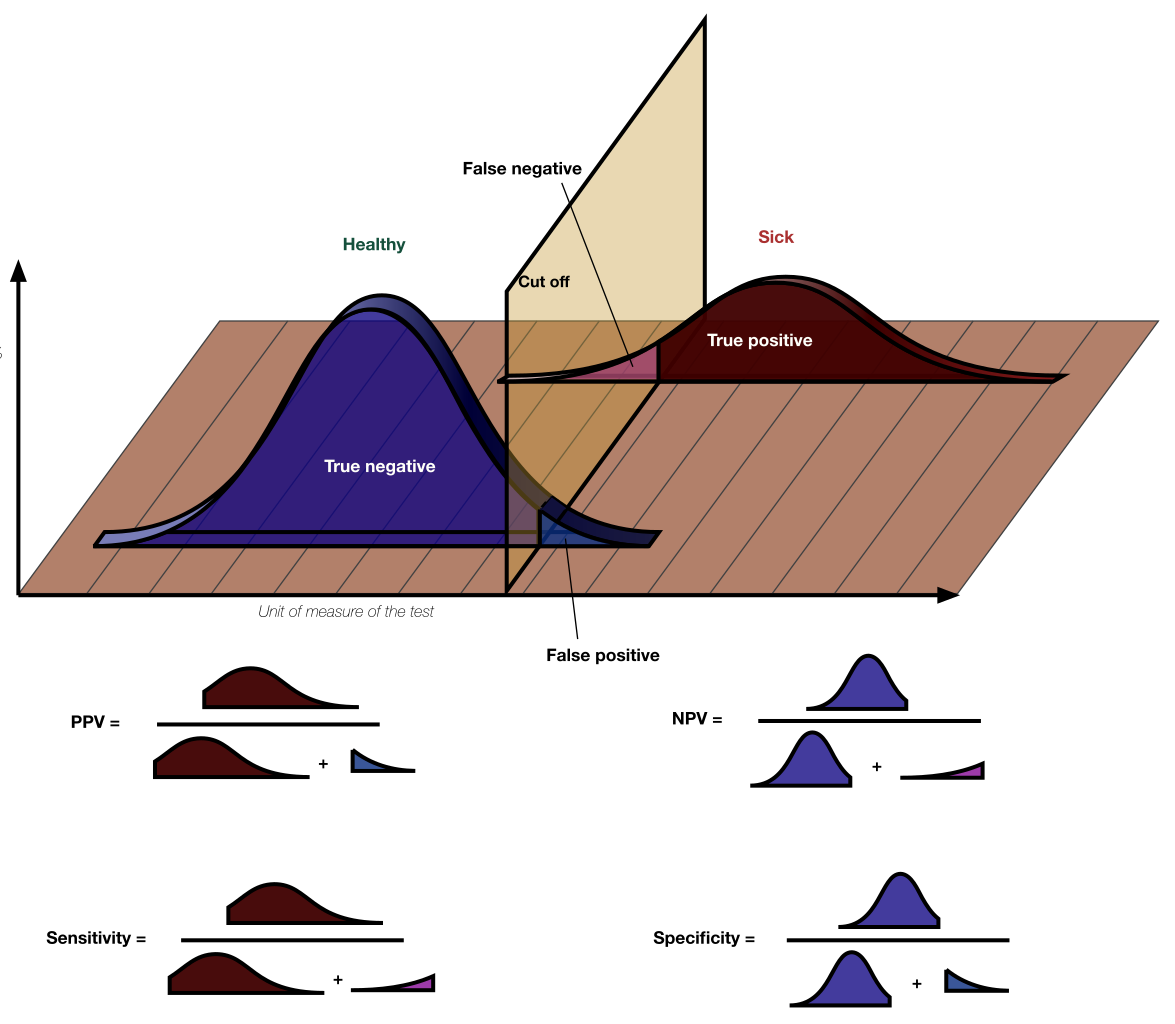
\includegraphics[width=0.75\textwidth]{images/stats.png}
\caption*{\tiny\color{Gray}%
Author: Luigi Albert Maria \\
License: CC BY-SA 4.0 \\
https://creativecommons.org/licenses/by-sa/4.0
}

\end{figure}


\end{frame}



%------------------------------------------%
% Question of the day
%------------------------------------------%

\section{Hypothesis}
\begin{frame}{Question and Hypothesis}

% Question of the day
\begin{center}
\begin{minipage}{.9\linewidth}
\begin{Block}{Question of the day.}

\vspace{.5\baselineskip}
\begin{itemize}

\item Can we find \underline{useful} accuracy statistics for our effects and aromas prediction model?

\end{itemize}

\vspace{.5\baselineskip}

\end{Block}
\end{minipage}
\end{center}

\end{frame}


%------------------------------------------%
% Methodology
%------------------------------------------%


%------------------------------------------%
% Results
%------------------------------------------%



%------------------------------------------%
% Conclusion
%------------------------------------------%


%------------------------------------------%
% Takeaway
%------------------------------------------%
\section{Takeaway}
\begin{frame}{}
\begin{center}

% Thank you.
\begin{minipage}{3.85in}
\begin{center}

\includegraphics[width=.25in]{images/prayer.png} {\Large \textbf{Thank you for coming.}}\\
\end{center}
\vspace*{0.5\baselineskip}

% Insight of the day.
\begin{center}
\begin{minipage}{\linewidth}
\begin{Block}{Insights of the Day}

\vspace{0.5\baselineskip}

\begin{itemize}

\item \underline{Sampling}, \underline{training}, and \underline{measuring} prediction accuracy helps to make your models robust.

\vspace{0.5\baselineskip}

\end{itemize}

\end{Block}
\end{minipage}
\end{center}

\vspace*{2\baselineskip}

\end{minipage}

\end{center}
\end{frame}
\end{document}
%------------------------------------------%
%------------------------------------------%